\documentclass[12pt, a4paper]{article}

% ==========================================
% 1. KHAI BÁO GÓI THƯ VIỆN (PACKAGES)
% ==========================================
% Bảng mã & Font chữ
\usepackage[utf8]{inputenc}
\usepackage[T5]{fontenc}

% Toán học
\usepackage{amsmath, amssymb}

% Căn lề & Bố cục trang
\usepackage[top=2.2cm, bottom=1.5cm, left=1cm, right=1cm, headheight=15pt]{geometry}
\usepackage{fancyhdr}
\usepackage{needspace}
\usepackage{tkz-tab}

% Đồ họa & Màu sắc
\usepackage{xcolor}
\usepackage{graphicx} 
\usepackage{tikz}
\usetikzlibrary{calc, shapes.geometric, positioning}


% Bảng biểu & Danh sách
\usepackage{colortbl}
\usepackage{array}
\usepackage{makecell}
\usepackage{multirow}
\usepackage{tasks}

% Biểu tượng
\usepackage{fontawesome5}

% ==========================================
% 2. THIẾT LẬP MÀU SẮC CHỦ ĐẠO
% ==========================================
\definecolor{goldyellow}{RGB}{255, 179, 0}
\definecolor{amberorange}{RGB}{230, 115, 0}
\definecolor{lightamber}{RGB}{255, 248, 225}
\definecolor{deepblue}{RGB}{25, 42, 86}
\definecolor{accentred}{RGB}{232, 65, 24}
\definecolor{softgray}{RGB}{220, 220, 222} 
\definecolor{fbblue}{RGB}{15, 80, 200}


% ==========================================
% 3. CẤU HÌNH HEADER & FOOTER
% ==========================================
\pagestyle{fancy}
\fancyhf{}
\renewcommand{\headrulewidth}{0pt}

% Khai báo biến lưu trữ nội dung góc phải của Header
\newcommand{\HeaderRightText}{}

% --- Header ---
\fancyhead[C]{
    \begin{tikzpicture}[remember picture, overlay]
        
        % Dải màu trang trí góc trên
        \path[fill=deepblue] (current page.north west) -- (current page.north east) 
            -- ($(current page.north east) + (0, -1.6cm)$) 
            .. controls ($(current page.north) + (3, -2.0cm)$) and ($(current page.north) + (-3, -0.4cm)$) .. 
            ($(current page.north west) + (0, -1.0cm)$) -- cycle;
            
        \path[fill=goldyellow] (current page.north west) -- (current page.north east) 
            -- ($(current page.north east) + (0, -1.0cm)$) 
            .. controls ($(current page.north) + (4, -1.0cm)$) and ($(current page.north) + (-2, -2.2cm)$) .. 
            ($(current page.north west) + (0, -1.6cm)$) -- cycle;
            
        \path[fill=amberorange] (current page.north west) -- ($(current page.north west) + (6.5cm, 0)$) 
            .. controls ($(current page.north west) + (4.5cm, -1.2cm)$) and ($(current page.north west) + (2cm, -2.0cm)$) .. 
            ($(current page.north west) + (0, -2.0cm)$) -- cycle;
            
        % Logo góc trái Header
        \node[anchor=west, inner sep=0pt] 
            at ($(current page.north west) + (0cm, -0.8cm)$) {
\includegraphics[height=2.0cm]{../../../image/logo-header.png}};
            
        % Text góc phải Header (Tự động lấy từ đối số thứ 3 của \titlebox)
        \node[anchor=east, text=white, font=\small\bfseries\sffamily] 
            at ($(current page.north east) + (-0.8cm, -0.5cm)$) {\HeaderRightText};
    \end{tikzpicture}
}

% --- Footer ---
\fancyfoot[C]{
    \begin{tikzpicture}[remember picture, overlay]
        % Đường kẻ ngang
        \draw[amberorange, line width=1.5pt] 
            ($(current page.south west) + (0cm, 0.4cm)$) -- ($(current page.south east) + (0cm, 0.4cm)$);

        % Dải cong góc phải
        \path[fill=goldyellow] (current page.south east) -- ($(current page.south east) + (-5cm, 0)$) 
            .. controls ($(current page.south east) + (-3cm, 0.8cm)$) and ($(current page.south east) + (-1.5cm, 1.2cm)$) .. 
            ($(current page.south east) + (0, 1.2cm)$) -- cycle;

        % Mạng xã hội
        \node[anchor=west, inner sep=0pt] at ($(current page.south west) + (1cm, 0.8cm)$) {
            \small\sffamily
            \textcolor{fbblue}{\faFacebook\hskip 4pt Toán Anh Huy MATH-STER}
            \hskip 18pt
            \textcolor{black}{\faTiktok\hskip 4pt huymathster}
        };

        % Số trang
        \node[circle, fill=white, draw=amberorange, line width=1.5pt, text=deepblue, font=\large\bfseries\sffamily, inner sep=4pt, minimum size=0.8cm] 
            at ($(current page.south east) + (-1.2cm, 0.6cm)$) {\thepage};
    \end{tikzpicture}
}

% ==========================================
% 4. ĐỊNH NGHĨA MACRO: KHUNG TIÊU ĐỀ
% ==========================================
\newcommand{\titlebox}[3]{
    % Gán nội dung đối số #3 vào biến HeaderRightText
    \gdef\HeaderRightText{#3}
    
    \begin{center}
    \vspace*{-0.5cm}
    \begin{tikzpicture}
        % Khung vô hình (Phantom Box) định chuẩn kích thước
        \node[text width=16cm, inner xsep=0pt, inner ysep=16pt, opacity=0] (MainBox) {
            \begin{minipage}[c]{4.2cm}
                \centering\vspace{0.1cm}
                \rule{2.2cm}{2.2cm} 
                \vspace{0.1cm}
            \end{minipage}%
            \begin{minipage}[c]{11.5cm}
                \centering\vspace{0.15cm}
                {\huge\bfseries\sffamily #2 \par}
                \vspace{0.15cm} 
            \end{minipage}
        };
        
        % Đổ bóng & Nền
        \fill[goldyellow, rounded corners=8pt] ([xshift=5pt, yshift=-5pt]MainBox.south west) rectangle ([xshift=5pt, yshift=-5pt]MainBox.north east);
        \fill[white, rounded corners=8pt] (MainBox.south west) rectangle (MainBox.north east);
        
        % Lưới ô ly & Nền Logo
        \begin{scope}
            \clip[rounded corners=8pt] (MainBox.south west) rectangle (MainBox.north east);
            \draw[step=0.4cm, softgray!50, line width=0.6pt] (MainBox.south west) grid (MainBox.north east);
            \fill[lightamber!60] (MainBox.south west) rectangle ([xshift=4.2cm]MainBox.north west);
        \end{scope}

        % Viền ngoài
        \draw[deepblue, line width=1.5pt, rounded corners=8pt] (MainBox.south west) rectangle (MainBox.north east);

        % Nội dung Text (Lớp trên cùng)
        \node[text width=16cm, inner xsep=0pt, inner ysep=16pt] at (MainBox.center) {
            \begin{minipage}[c]{4.2cm}
                \centering
                % --- ĐIỀU CHỈNH TỌA ĐỘ LOGO Ở ĐÂY ---
                \hspace*{-0.5cm}\raisebox{-0.2cm}{
\includegraphics[width=5.5cm]{../../../image/logo.png}}
            \end{minipage}%
            \begin{minipage}[c]{11.5cm}
                \centering\vspace{0.15cm}
                {\huge\bfseries\sffamily\color{deepblue} #2 \par}
                \vspace{0.15cm} 
            \end{minipage}
        };
        
        % Trang trí phụ kiện
        \draw[deepblue, line width=1.5pt, dashed] ([xshift=4.2cm]MainBox.north west) -- ([xshift=4.2cm]MainBox.south west);
        \node[regular polygon, regular polygon sides=4, rotate=45, fill=white, draw=accentred, line width=1.2pt, inner sep=2.5pt] at ([xshift=4.2cm]MainBox.west) {};
        \node[anchor=west, fill=amberorange, text=white, font=\large\bfseries\sffamily, rounded corners=4pt, draw=deepblue, line width=1.5pt, inner xsep=12pt, inner ysep=6pt] at ([xshift=1.5cm]MainBox.north west) {#1};
        \fill[accentred] ([xshift=-1.8cm, yshift=-0.4cm]MainBox.north east) circle (3pt);
        \fill[amberorange] ([xshift=-1.4cm, yshift=-0.4cm]MainBox.north east) circle (3pt);
        \fill[goldyellow] ([xshift=-1.0cm, yshift=-0.4cm]MainBox.north east) circle (3pt);
    \end{tikzpicture}
    \vspace*{0cm}
    \end{center}
}

% ==========================================
% 5. ĐỊNH NGHĨA MACRO: CẤU TRÚC CÂU HỎI (ÉP SÁT NHAU)
% ==========================================
\newcommand{\questioncore}[2]{
    % Xóa khoảng cách phía trên, ép sát câu trước
    \noindent \textbf{\textcolor{deepblue}{Câu #1.} \textcolor{accentred}{[STER]}} #2
    \par\nopagebreak
}

% Cấu hình hiển thị đáp án trắc nghiệm
\settasks{
    label=\textbf{\textcolor{amberorange}{\Alph*.}}, 
    label-width=15pt,     
    item-indent=25pt,     
    label-offset=6pt,    
    column-sep=20pt,     
    after-item-skip=2pt  % Đã giảm tối đa khoảng cách giữa các dòng đáp án A B C D
}

% Hàm vẽ dòng kẻ nháp
\newcommand{\drawdashlines}[1]{
    \ifnum#1>0
        \nopagebreak\vspace{0.1cm}\noindent 
        \begin{tikzpicture}
            \foreach \i in {1,...,#1} {
                \draw[softgray, line width=0.2pt] (0,-{\i*0.75}) -- (\textwidth-4pt,-{\i*0.75});
            }
        \end{tikzpicture}
        \par
    \fi
    % Đã xóa hoàn toàn khoảng cách thừa ở nhánh else
}

% --- Dạng 1: Trắc nghiệm 4 đáp án ---
\newcommand{\questionLinesManual}[4]{
    \pgfmathsetmacro{\calculatedSpace}{1.5 + #1 * 0.65}
    \needspace{\calculatedSpace cm} 
    \questioncore{#2}{#3}
    #4
    \par\nopagebreak
    \drawdashlines{#1}
}

% --- Dạng 2: Trắc nghiệm Đúng/Sai ---
\newcommand{\questionTrueFalse}[4]{
    \pgfmathsetmacro{\calculatedSpace}{3.0 + #1 * 0.65} 
    \needspace{\calculatedSpace cm}
    \questioncore{#2}{#3}
    
    \nopagebreak
    \begin{center}
    \renewcommand{\arraystretch}{1.2} % Bóp nhỏ chiều cao của bảng Đ/S
    \begin{tabular}{|>{\centering\arraybackslash}m{0.8cm}|m{12cm}|>{\centering\arraybackslash}m{2cm}|>{\centering\arraybackslash}m{2cm}|}
        \hline
        \rowcolor{amberorange!20}
        & \multicolumn{1}{>{\centering\arraybackslash}m{12cm}|}{\textbf{\textcolor{deepblue}{Mệnh đề}}} & 
        \textbf{\textcolor{deepblue}{Đúng}} & 
        \textbf{\textcolor{deepblue}{Sai}} \\
        \hline
        #4
        \hline
    \end{tabular}
    \renewcommand{\arraystretch}{1}
    \end{center}
    
    \par\nopagebreak
    \drawdashlines{#1}
}

% ----- Dạng 3: Tự luận ngắn -----
\newcommand{\questionShortAnswer}[3]{
    \pgfmathsetmacro{\calculatedSpace}{1.5 + #1 * 0.8}
    \needspace{\calculatedSpace cm}
    
    {\linespread{1.1}\selectfont % Bóp nhỏ giãn dòng của câu tự luận
    \questioncore{#2}{#3}\par}
    
    \nopagebreak
    \begin{flushright}
        \begin{tikzpicture}
            \node[anchor=east, font=\small\bfseries\sffamily, text=deepblue] 
                at (-0.2, 0.4) {Đáp án:};
            \fill[goldyellow, rounded corners=3pt] (0.08, -0.08) rectangle (3.08, 0.72);
            \draw[draw=deepblue, fill=white, line width=1.2pt, rounded corners=3pt] 
                (0,0) rectangle (3.0, 0.8);
            \foreach \x in {0.75, 1.5, 2.25} {
                \draw[draw=deepblue, line width=0.6pt] (\x, 0) -- (\x, 0.8);
            }
        \end{tikzpicture}
    \end{flushright}
    
    \par\nopagebreak
    \drawdashlines{#1}
}

% ==========================================
% BẮT ĐẦU NỘI DUNG TÀI LIỆU
% ==========================================
\begin{document}

% Truyền 3 tham số: {Nhãn cam} {Chữ to chính giữa} {Chữ ở góc phải Header}
\titlebox{Chủ đề: Hàm số}{Bài tập giá trị lớn nhất - giá trị nhỏ nhất}{Hàm số: GTLN - GTNN}
\questionLinesManual{0}{1}{ Cho hàm số \( f(x) \) liên tục trên \([-1; 5]\) và có đồ thị trên đoạn \([-1; 5]\) như hình vẽ bên dưới. Tổng giá trị lớn nhất và giá trị nhỏ nhất của hàm số \( f(x) \) trên đoạn \([-1; 5]\) bằng

\begin{center}
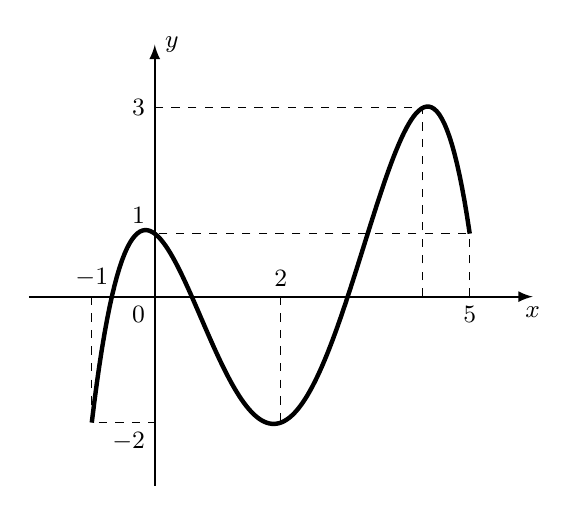
\begin{tikzpicture}[>=latex, scale=0.8]
    % 1. Hệ trục tọa độ Ox, Oy màu đen
    \draw[->, black, thick] (-2,0) -- (6,0) node[below] {\small $x$};
    \draw[->, black, thick] (0,-3) -- (0,4) node[right] {\small $y$};
    \node[below left] at (0,0) {\small $0$};
    
    % 2. Đồ thị hàm số màu đen
    \draw[black, ultra thick, samples=150, domain=-1:5] 
plot (\x, {-0.1588135590717*\x*\x*\x*\x + 1.2862146877635*\x*\x*\x - 2.3097740105484*\x*\x - 0.7548022573836*\x + 1});
    % 3. Các đường nét đứt và nhãn tọa độ màu đen
    % Tại x = -1, y = -2
    \draw[dashed, black] (-1,0) -- (-1,-2) -- (0,-2);
    \node[above] at (-1,0) {\small $-1$};
    \node[below left] at (0,-2) {\small $-2$};
    
    % Tại x = 0, y = 1
    \node[above left] at (0,1) {\small $1$};
    
    % Tại x = 2, y = -2
    \draw[dashed, black] (2,0) -- (2,-2);
    \node[above] at (2,0) {\small $2$};
    
    % Tại đỉnh cực đại thứ hai (x ≈ 4.25, y = 3)
    \draw[dashed, black] (4.25,0) -- (4.25,3) -- (0,3);
    \node[left] at (0,3) {\small $3$};
    
    % Tại điểm cuối cùng x = 5, y = 1
    \draw[dashed, black] (5,0) -- (5,1) -- (0,1);
    \node[below] at (5,0) {\small $5$};

\end{tikzpicture}
\end{center}

}{
    \begin{tasks}(4)
        \task $-1$
        \task $4$
        \task $1$
        \task $2$
    \end{tasks}
}

\questionLinesManual{0}{2}{ Cho hàm số \( y = f(x) \) liên tục trên đoạn \([-2;6]\) và có đồ thị như hình vẽ bên dưới.

\begin{center}
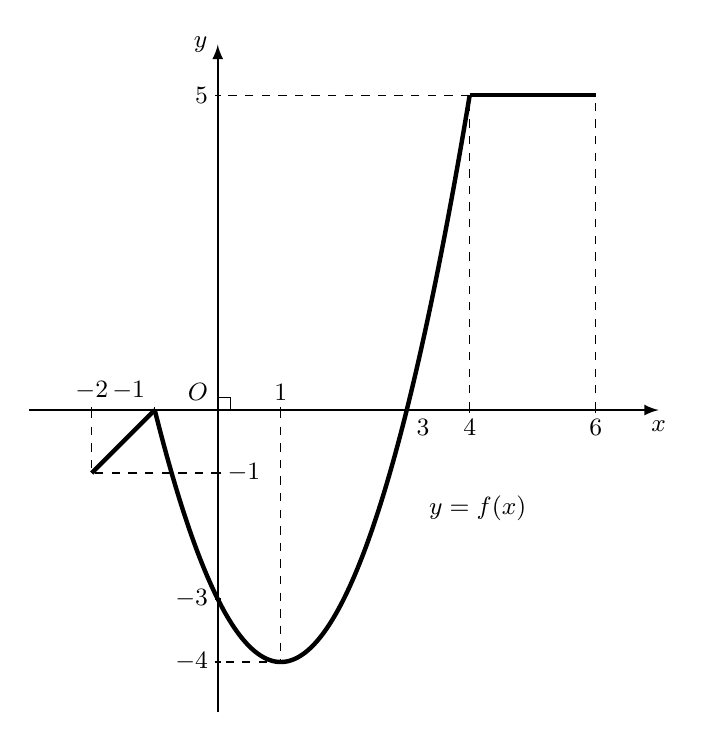
\begin{tikzpicture}[>=latex, scale=0.8]
    % 1. Hệ trục tọa độ Ox, Oy màu đen và ký hiệu vuông góc
    \draw[->, black, thick] (-3,0) -- (7,0) node[below] {\small $x$};
    \draw[->, black, thick] (0,-4.8) -- (0,5.8) node[left] {\small $y$};
    \node[above left] at (0,0) {\small $O$};
    \draw[black] (0,0.2) -- (0.2,0.2) -- (0.2,0); % Ký hiệu vuông góc tại gốc O

    % Các vạch nhỏ chia tọa độ trên trục Ox và Oy
    \foreach \x in {-2, -1, 1, 3, 4, 6} \draw[black] (\x, 0.05) -- (\x, -0.05);
    \foreach \y in {-4, -3, -1, 5} \draw[black] (0.05, \y) -- (-0.05, \y);

    % 2. Đồ thị hàm số màu đen gồm các nhánh liền mạch
    % Nhánh 1: Đoạn thẳng từ (-2, -1) lên (-1, 0)
    \draw[black, ultra thick] (-2,-1) -- (-1,0);
    
    % Nhánh 2: Parabol từ (-1, 0) qua (0, -3), đạt cực tiểu tại (1, -4) rồi đi lên cắt Ox tại x = 3 đến điểm (4, 5)
    \draw[black, ultra thick, samples=150, domain=-1:4] plot (\x, {\x*\x - 2*\x - 3});
    
    % Nhánh 3: Đoạn thẳng nằm ngang từ (4, 5) đến điểm mút (6, 5)
    \draw[black, ultra thick] (4,5) -- (6,5);
    
    % Nhãn tên đồ thị y = f(x)
    \node[below right] at (3.2,-1.2) {\small $y = f(x)$};

    % 3. Các đường nét đứt và nhãn tọa độ màu đen
    % Tại mốc x = -2, y = -1
    \draw[dashed, black] (-2,0) -- (-2,-1) -- (0,-1);
    \node[above] at (-2,0) {\small $-2$};
    \node[above left] at (-1,0) {\small $-1$};
    \node[right] at (0,-1) {\small $-1$};
    
    % Tại vị trí cắt trục tung Oy tại y = -3
    \node[left] at (0,-3) {\small $-3$};
    
    % Tại cực tiểu x = 1, y = -4
    \draw[dashed, black] (1,0) -- (1,-4) -- (0,-4);
    \node[above] at (1,0) {\small $1$};
    \node[left] at (0,-4) {\small $-4$};
    
    % Tại vị trí cắt trục hoành x = 3
    \node[below right] at (3,0) {\small $3$};
    
    % Tại mốc x = 4, y = 5
    \draw[dashed, black] (4,0) -- (4,5) -- (0,5);
    \node[below] at (4,0) {\small $4$};
    \node[left] at (0,5) {\small $5$};
    
    % Tại điểm cuối cùng x = 6, y = 5
    \draw[dashed, black] (6,0) -- (6,5);
    \node[below] at (6,0) {\small $6$};

\end{tikzpicture}
\end{center}

Gọi \( M \) và \( m \) lần lượt là giá trị lớn nhất và nhỏ nhất của hàm số đã cho trên đoạn \([-2;6]\). Giá trị của \( M - m \) bằng}{
    \begin{tasks}(4)
        \task $9$
        \task $-8$
        \task $-9$
        \task $8$
    \end{tasks}
}

\questionLinesManual{0}{3}{Cho hàm số \( y = f(x) \) liên tục và có đồ thị trên đoạn \([-2; 4]\) như hình vẽ bên. Tổng giá trị lớn nhất và nhỏ nhất của hàm số \( y = f(x) \) trên đoạn \([-2; 4]\) bằng

\begin{center}
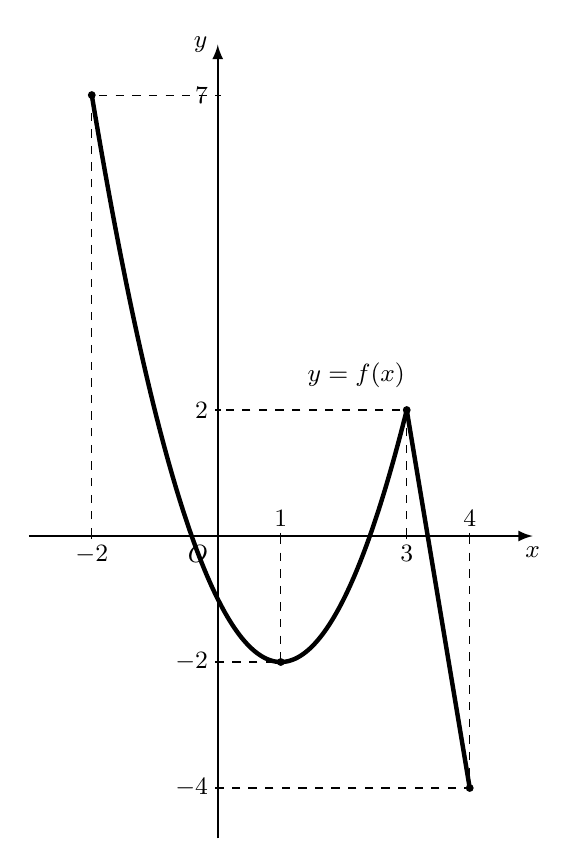
\begin{tikzpicture}[>=latex, scale=0.8]
    % 1. Hệ trục tọa độ Ox, Oy màu đen
    \draw[->, black, thick] (-3,0) -- (5,0) node[below] {\small $x$};
    \draw[->, black, thick] (0,-4.8) -- (0,7.8) node[left] {\small $y$};
    \node[below left] at (0,0) {\small $O$};

    % Các vạch nhỏ chia tọa độ trên trục Ox và Oy
    \foreach \x in {-2, 1, 3, 4} \draw[black] (\x, 0.05) -- (\x, -0.05);
    \foreach \y in {-4, -2, 2, 7} \draw[black] (0.05, \y) -- (-0.05, \y);

    % 2. Đồ thị hàm số màu đen gồm các nhánh liền mạch
    % Nhánh 1: Parabol/đường cong từ (-2, 7) đi xuống đạt cực tiểu tại (1, -2) rồi đi lên cực đại nhọn tại (3, 2)
    % Hàm mẫu phù hợp cho cung này: y = (x-1)^2 - 2 trên đoạn [-2, 3]
    \draw[black, ultra thick, samples=150, domain=-2:3] plot (\x, {(\x-1)*(\x-1) - 2});
    
    % Nhánh 2: Đoạn thẳng dốc xuống từ cực đại nhọn (3, 2) đến điểm mút (4, -4)
    \draw[black, ultra thick] (3,2) -- (4,-4);

    % Vẽ các điểm mút tròn tại các vị trí giới hạn (giữ màu đen đồng bộ)
    \filldraw[black] (-2,7) circle (1.5pt);
    \filldraw[black] (1,-2) circle (1.5pt);
    \filldraw[black] (3,2) circle (1.5pt);
    \filldraw[black] (4,-4) circle (1.5pt);

    % Tên đồ thị y = f(x)
    \node[above] at (2.2,2.2) {\small $y = f(x)$};

    % 3. Các đường nét đứt và nhãn tọa độ màu đen
    % Tại mốc x = -2, y = 7
    \draw[dashed, black] (-2,0) -- (-2,7) -- (0,7);
    \node[below] at (-2,0) {\small $-2$};
    \node[left] at (0,7) {\small $7$};
    
    % Tại mốc cực tiểu x = 1, y = -2
    \draw[dashed, black] (1,0) -- (1,-2) -- (0,-2);
    \node[above] at (1,0) {\small $1$};
    \node[left] at (0,-2) {\small $-2$};
    
    % Tại mốc cực đại nhọn x = 3, y = 2
    \draw[dashed, black] (3,0) -- (3,2) -- (0,2);
    \node[below] at (3,0) {\small $3$};
    \node[left] at (0,2) {\small $2$};
    
    % Tại mốc điểm mút cuối x = 4, y = -4
    \draw[dashed, black] (4,0) -- (4,-4) -- (0,-4);
    \node[above] at (4,0) {\small $4$};
    \node[left] at (0,-4) {\small $-4$};

\end{tikzpicture}
\end{center}

}{
    \begin{tasks}(4)
        \task $5$
        \task $3$
        \task $0$
        \task $-2$
    \end{tasks}
}

\questionLinesManual{0}{4}{ Cho hàm số \( y = f(x) \) có bảng biến thiên như sau

\begin{center}
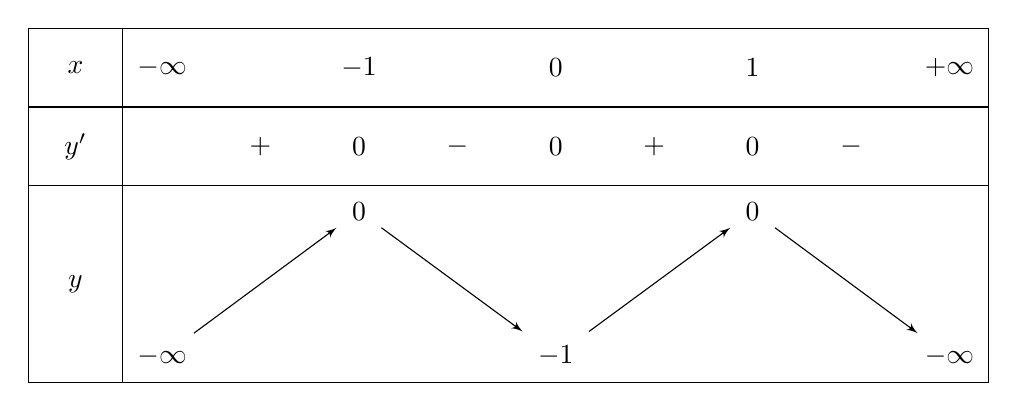
\begin{tikzpicture}[>=stealth]
    % Khởi tạo bảng biến thiên với độ rộng cột tiêu đề và khoảng cách giữa các cột số
    \tkzTabInit[nocadre=false, lgt=1.2, espcl=2.5]
        {$x$ / 1, $y'$ / 1, $y$ / 2.5}                    % Tên dòng / Chiều cao dòng
        {$-\infty$, $-1$, $0$, $1$, $+\infty$}            % Các giá trị trên dòng x
    
    % Xét dấu của đạo hàm y' (+, 0, -, 0, +, 0, -)
    \tkzTabLine{ , +, 0, -, 0, +, 0, - }
    
    % Sự biến thiên và các giá trị cực trị của hàm số y
    \tkzTabVar{-/ $-\infty$, +/ $0$, -/ $-1$, +/ $0$, -/ $-\infty$}
\end{tikzpicture}
\end{center}

Khẳng định nào sau đây sai?}{
    \begin{tasks}(1)
        \task Hàm số \( y = f(x) \) nghịch biến trên \((-1; 0)\) và \((1; +\infty)\).
        \task Giá trị nhỏ nhất của hàm số \( y = f(x) \) trên tập \( \mathbb{R} \) bằng \(-1\).
        \task Giá trị lớn nhất của hàm số \( y = f(x) \) trên tập \( \mathbb{R} \) bằng \(0\).
        \task Đồ thị hàm số \( y = f(x) \) không có đường tiệm cận.
    \end{tasks}
}

\questionLinesManual{0}{5}{ Cho hàm số \( y = f(x) \) xác định trên \( \mathbb{R} \) và có bảng xét dấu \( f'(x) \) như sau:

\begin{center}
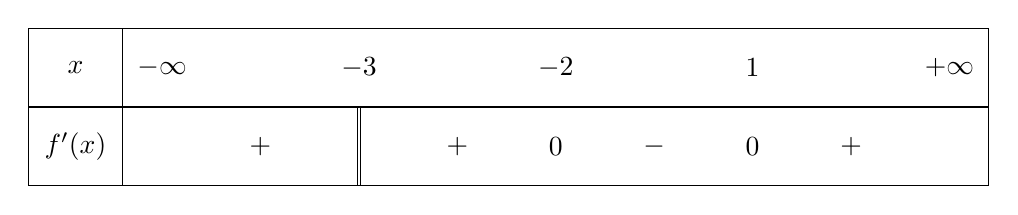
\begin{tikzpicture}[>=stealth]
    % Khởi tạo bảng xét dấu gồm 2 dòng: x và f'(x)
    \tkzTabInit[nocadre=false, lgt=1.2, espcl=2.5]
        {$x$ / 1, $f'(x)$ / 1}                            % Tên dòng / Chiều cao dòng
        {$-\infty$, $-3$, $-2$, $1$, $+\infty$}           % Các giá trị trên dòng x
    
    % Xét dấu của đạo hàm f'(x), sử dụng 'd' tại x = -3
    \tkzTabLine{ , +, d, +, 0, -, 0, + }
\end{tikzpicture}
\end{center}

Khẳng định nào dưới đây đúng?}{
    \begin{tasks}(4)
        \task \(\min\limits_{(-2;+\infty)} f(x) = f(1)\)
        \task \(\min\limits_{(-\infty;-3]} f(x) = f(-3)\)
        \task \(\min\limits_{(-2;1)} f(x) = f(1)\)
        \task \(\min\limits_{[-3;-2]} f(x) = f(-2)\)
    \end{tasks}
}

\questionLinesManual{0}{6}{ Cho hàm số \( y = f(x) \) liên tục và có bảng biến thiên trên đoạn \([-1; 3]\) như hình vẽ bên. Khẳng định nào sau đây đúng?

\begin{center}
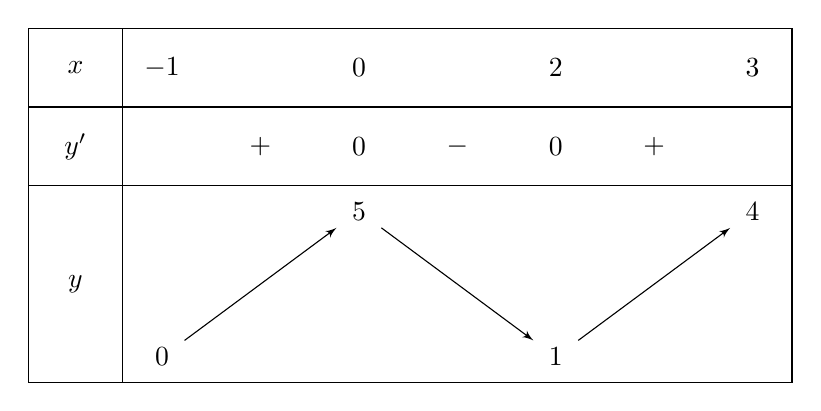
\begin{tikzpicture}[>=stealth]
    % Khởi tạo bảng biến thiên với độ rộng cột tiêu đề và khoảng cách giữa các số
    \tkzTabInit[nocadre=false, lgt=1.2, espcl=2.5]
        {$x$ / 1, $y'$ / 1, $y$ / 2.5}         % Tên các dòng và chiều cao tương ứng
        {$-1$, $0$, $2$, $3$}                  % Các giá trị trên dòng x
    
    % Xét dấu của đạo hàm y'
    \tkzTabLine{ , +, 0, -, 0, + }
    
    % Điền các mũi tên biến thiên và giá trị tương ứng của hàm số y
    \tkzTabVar{-/ $0$, +/ $5$, -/ $1$, +/ $4$}
\end{tikzpicture}
\end{center}

}{
    \begin{tasks}(4)
        \task \(\max\limits_{[-1;3]} f(x) = f(0)\).
        \task \(\max\limits_{[-1;3]} f(x) = f(3)\).
        \task \(\max\limits_{[-1;3]} f(x) = f(2)\).
        \task \(\max\limits_{[-1;3]} f(x) = f(-1)\).
    \end{tasks}
}

\questionLinesManual{0}{7}{ Gọi \( M, m \) lần lượt là giá trị lớn nhất và giá trị nhỏ nhất của hàm số \( f(x) = x^4 - 2x^2 - 1 \) trên đoạn \([-1; 2]\). Giá trị của biểu thức \( M + 3m \) bằng}{
    \begin{tasks}(4)
        \task $1$
        \task $5$
        \task $6$
        \task $4$
    \end{tasks}
}

\questionLinesManual{0}{8}{ Giá trị lớn nhất \( M \) của hàm số \( y = x^3 + 3x^2 - 9x - 6 \) trên đoạn \([-1; 2]\) là?}{
    \begin{tasks}(4)
        \task \( M = 7 \)
        \task \( M = 5 \)
        \task \( M = -11 \)
        \task \( M = 21 \)
    \end{tasks}
}

\questionLinesManual{0}{9}{Giá trị lớn nhất của hàm số \( y = \sqrt{4 - x^2} \) là}{
    \begin{tasks}(4)
        \task $2$
        \task $0$
        \task $4$
        \task $1$
    \end{tasks}
}

\questionLinesManual{0}{10}{ Tìm giá trị lớn nhất của hàm số \( f(x) = \sin x + 3 \)  là}{
    \begin{tasks}(4)
        \task \(\dfrac{9}{8}\)
        \task $4$
        \task $2$
        \task $1$
    \end{tasks}
}


\end{document}